\section{eo\-MOFitness\-Stat$<$ EOT, Part\-Fit\-T $>$ Class Template Reference}
\label{classeo_m_o_fitness_stat}\index{eoMOFitnessStat@{eoMOFitnessStat}}
For multi-objective fitness, we need to translate a stat$<$vector$<$double$>$ $>$ into a vector$<$stat$>$, so each objective gets a seperate stat.  


{\tt \#include $<$eo\-MOFitness\-Stat.h$>$}

Inheritance diagram for eo\-MOFitness\-Stat$<$ EOT, Part\-Fit\-T $>$::\begin{figure}[H]
\begin{center}
\leavevmode
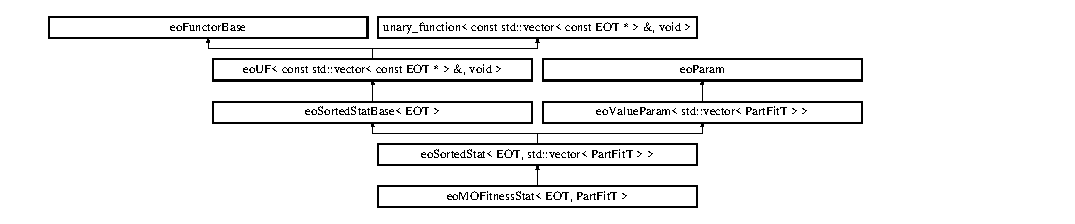
\includegraphics[height=2.55708cm]{classeo_m_o_fitness_stat}
\end{center}
\end{figure}
\subsection*{Public Member Functions}
\begin{CompactItemize}
\item 
{\bf eo\-MOFitness\-Stat} (unsigned \_\-objective, std::string \_\-description=\char`\"{}MO-Fitness\char`\"{})\label{classeo_m_o_fitness_stat_a0}

\begin{CompactList}\small\item\em Ctor: say what component you want. \item\end{CompactList}\item 
virtual void {\bf operator()} (const std::vector$<$ const {\bf EOT} $\ast$ $>$ \&\_\-pop\-Pters)\label{classeo_m_o_fitness_stat_a1}

\begin{CompactList}\small\item\em The pure virtual function that needs to be implemented by the subclass. \item\end{CompactList}\end{CompactItemize}
\subsection*{Private Attributes}
\begin{CompactItemize}
\item 
unsigned int {\bf objective}\label{classeo_m_o_fitness_stat_r0}

\end{CompactItemize}


\subsection{Detailed Description}
\subsubsection*{template$<$class EOT, class Part\-Fit\-T = double$>$ class eo\-MOFitness\-Stat$<$ EOT, Part\-Fit\-T $>$}

For multi-objective fitness, we need to translate a stat$<$vector$<$double$>$ $>$ into a vector$<$stat$>$, so each objective gets a seperate stat. 



Definition at line 64 of file eo\-MOFitness\-Stat.h.

The documentation for this class was generated from the following file:\begin{CompactItemize}
\item 
eo\-MOFitness\-Stat.h\end{CompactItemize}
